% author:         zhangyi zju_cs
% course:         生物智能与算法
% teacher:        yuanxi
% environment:    ubuntu 16.04
%                 texlive-full
%                 texlive-xetex
% editor:         vscode
%                 latex-workshop
% compiler:       xelatex
%                 bibtex

\documentclass[a4paper]{article}

\usepackage{ctex}           % support chinese
\usepackage{geometry}       % setting margin
\usepackage{setspace}       % setting space
\usepackage{algorithm}      % support pseudocode
\usepackage{algpseudocode}  % support pseudocode
\usepackage{caption}        % support caption
\usepackage{amsmath}        % support newtheorem
\usepackage{graphicx}       % support insert iamge

\newtheorem{definition}{\hspace{2em}定义}


\title{多种群协同进化}
\date{2018-04-30}
\author{张毅}

\geometry{left=3.5cm,right=3.5cm,top=4.5cm,bottom=4.5cm}
\setcounter{tocdepth}{2}
\doublespacing

\begin{document}
    
    \pagenumbering{gobble}
    \maketitle


    \newpage
    \tableofcontents
    

    \newpage
    \pagenumbering{arabic}
    \section{引言}

    演化算法(Evolutionary algorithm, EA)是模拟生物遗传进化规律的一类启发式算法。由于其整体搜索策略和优化计算不依赖梯度信息,相比其他传统的局部搜索启发式算法,演化算法在搜索空间高度模态化,不连续或高度受限时具有明显优势。演化算法具有自组织、自适应、自学习的特性,能够不受问题性质的限制,有效地处理传统优化算法难以解决的复杂问题\cite{sun_ea}。但是,演化算法也存在一些限制:1)当问题的搜索空间非常大,其定义为两个或者多个互相交互的子空间的笛卡尔乘积时,演化算法很难进行有效的搜索。在极端的情况下,搜索空间可能会无限大,演化算法的搜索需要能够聚焦在相关的区域中。2)当没有内在的客观度量来评估个体适应度时演化算法很难适用。比如:不断演变的游戏策略。3)在搜索复杂结构的空间时,如果没有进行特定域的修改来帮助指导搜索,演化算法也很难适用。为解决演化算法存在的问题,协同演化算法被提出来。
    
    协同演化算法(Coevolutionary algorithm, CEA)是演化算法的扩展,相比演化算法,其个体适应度的计算是主观的,根据他们与其他个体的相交互来评估的,交互伙伴可以是同一种群的个体或者不同种群的个体\cite{wiegand2003analysis}。根据交互的性质,协同演化算法可以分为两大类:竞争型协同进化算法与合作型协同进化算法。对于合作型协同演化算法,个体如果与其他个体一起协作良好将获得奖励,协作不佳则受到惩罚。例如,在一个协同演化算法中,每个种群代表一个大问题的一个子问题,合作演化的任务就是每个种群为了解决大问题而演化出越来越适合的子问题的解。对于竞争型协同进化算法,个体获得的奖励是与他们互动的个体付出的代价。例如,捕食-被捕食模型中,其中一个种群中的个体代表某种设备(例如,排序网络),另一个种群中的个体代表该设备的输入(例如,数据),第一个种群中个体的目标是发展越来越好的设备来处理输入,而第二群人的目标是为该设备演化出越来越难的输入。


    \newpage
    \section{相关研究}
    
    1991年,Hillis等人首次对具有捕食-被捕食关系的两个对立种群(排序网络与数据集)进行协同演化\cite{hillis1990co}。其中,在第一个种群中的每个个体代表一个潜在的排序网络,其适应度的计算依赖于它对‘数据集’种群的排序效果。在另一个种群中的每个个体代表一个潜在的数据集,其适应度的计算依赖于混淆‘排序网络’种群的程度。
    
    在过去的研究中,竞争型协同演化算法在协同演化算法中占主导地位,其被广泛应用于游戏策略领域\cite{rosin1995methods,pollack1998co}。1993年,Angeline和Pollack提出竞争适应度的概念来提供比独立适应度函数更加鲁棒的训练环境,其展示了竞争对演化过程的有效性。1994年,Schlierkamp-Voosen等人成功地将竞争型协同演化应用于他们的育种遗传算法。当前,竞争型协同进化算法也已经被应用于各种机器学习问题。
    
    1994年,Potter和De Jong为研究合作型协同演化算法打开了大门\cite{potter1994cooperative},他们为这种模型开发了一个相对一般的框架,并首先应用于静态函数优化,其后又将其应用于神经网络学习。在Potter的模型中,每个种群都包含代表一个大问题中某个子问题的个体,这些种群的进化几乎是独立发生的,彼此协调,相互作用只是为了计算适应性。这样的过程可以是静态的,其子问题的划分是事先确定的且从不会改变,或者也可以是动态的,其在运行过程中可以添加或移除子问题的数量。1997年,Eriksson和Olsson使用合作协同进化算法进行库存控制优化。


    \newpage
    \section{协同进化算法}

    本章的开始,我们首先给出协同演化算法的定义。
    
    \begin{definition}
        协同演化算法:协同演化算法一种演化算法,其中个体的适应度其与其他个体相互作用的主观函数。
    \end{definition}

    \begin{figure}[H]
        \centering
        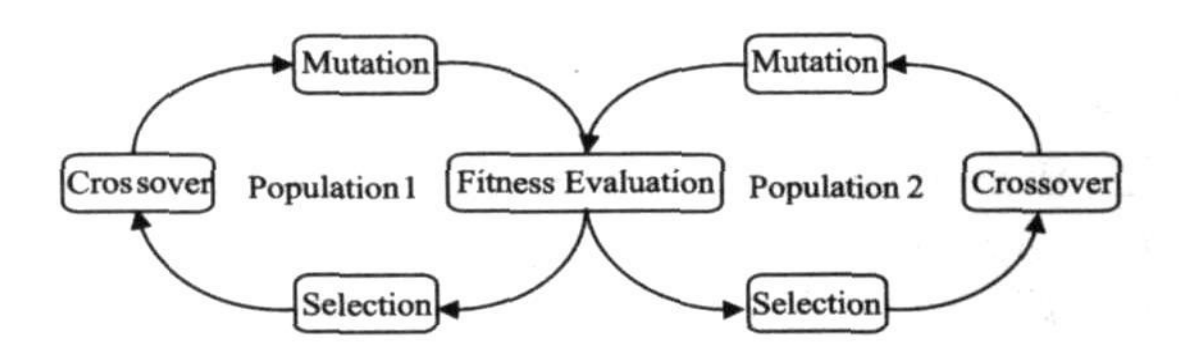
\includegraphics[width=0.8\linewidth]{./images/cea_framework.png}
        \caption{The overall framework of CEA}
        \label{fig:cea_framework}
    \end{figure}
    
    \begin{algorithm}
        
        \caption{the framework of Coevolutionary algorithm}
        \label{alg1}

        \begin{algorithmic}[1]
            \State $a$
        \end{algorithmic}

    \end{algorithm}

    \subsection{适应度计算}
    
    \subsection{交互方法}
    
    对于协同演化算法,个体在适应度评估时,如何选择与其交互的竞争或合作者非常重要。一种最容易想到的方式是选择所有可能的合作或竞争者与其进行交互。这种方式通常成为“完全匹配”。另一个极端是个体在进行适应度评估时只与一名竞争或合作者进行交互。这种方式的一个重要问题是如何选择这个竞争或合作者。除了这两种极端的做法,还有一种就是选择竞争或合作者的某个子集与其进行交互。子集的选择可以采用随机选择或者其他方法。

    对于交互对象的选择,往往是适应度评估效果与交互计算代价的折中。对于“完全匹配”方式,每个个体的适应度计算需要与所有可能的合作或竞争者的参与,这种方式往往使适应度的计算更加可信,但是它所带来的计算代价非常大,当个体数目很大的时候,这种方式会明显增加算法的时间复杂度。而对于只选择一个竞争或合作者进行交互的方式,虽然它的计算代价非常小,但是个体适应度的计算往往与选择的交互对象直接相关,鲁棒性差。通常,折中的方式被大多数协同演化算法选择。

    \subsection{竞争型协同进化算法}

    \subsection{合作型协同进化算法}

    \newpage
    \section{协同进化算法的缺点}

    \newpage
    \bibliography{cea}
    \bibliographystyle{ieeetr}

\end{document}